% !TeX root = ../../../master.tex

\subsection{Umfrage erstellen}
\label{ssec:UmfrageErstellen}

Das Herzstück der Applikation soll das Erstellen einer Umfrage sein. 
Hier soll der Benutzer die Möglichkeit haben, eine Umfrage zu erstellen, die verschiedene Fragetypen beinhaltet. 
Fragetypen sind exemplarisch: 
%
\begin{itemize}
	\item Freitext (Single Input)
	\item Checkbox, Matrix (Multiple Choice)
	\item Radiogroup, Marix (Single Choice)
	\item Dropdown 
	\item Rating (Bewerung Skala)
	\item Boolean (Ja/Nein)
	\item Datepicker (Datumsfelder)
\end{itemize}
%

Wie der \abb \myRefGeneral{fig:SurveyCreatorImplement} stellt den Umfrageeditor der Anwendung dar. In diesem kann der Benutzer seine Umfragen erstellen sowie editieren kann. 
Der Benutzer gibt der Umfrage einen Titel engl{title} sowie eine Beschreibung \engl{description}. 
Er kann mehrere Seiten anlegen und auch jeder Seite eine \emph{title} und \emph{description} geben. \newline
Über die Toolbox (linke Seite) kann der Benutzer über \emph{Drag \& Drop} die verschiedene Fragetypen auf die ausgewählte Seite schieben. \todo{evtl. neues Bild mit versch. FrageTpen} 
Hier kann der Benutzer die Frage definieren und mögliche Auswahlmöglichkeiten (bei Single/Multiple Choice) definieren. 

\begin{figure}[hp]
	\centering
	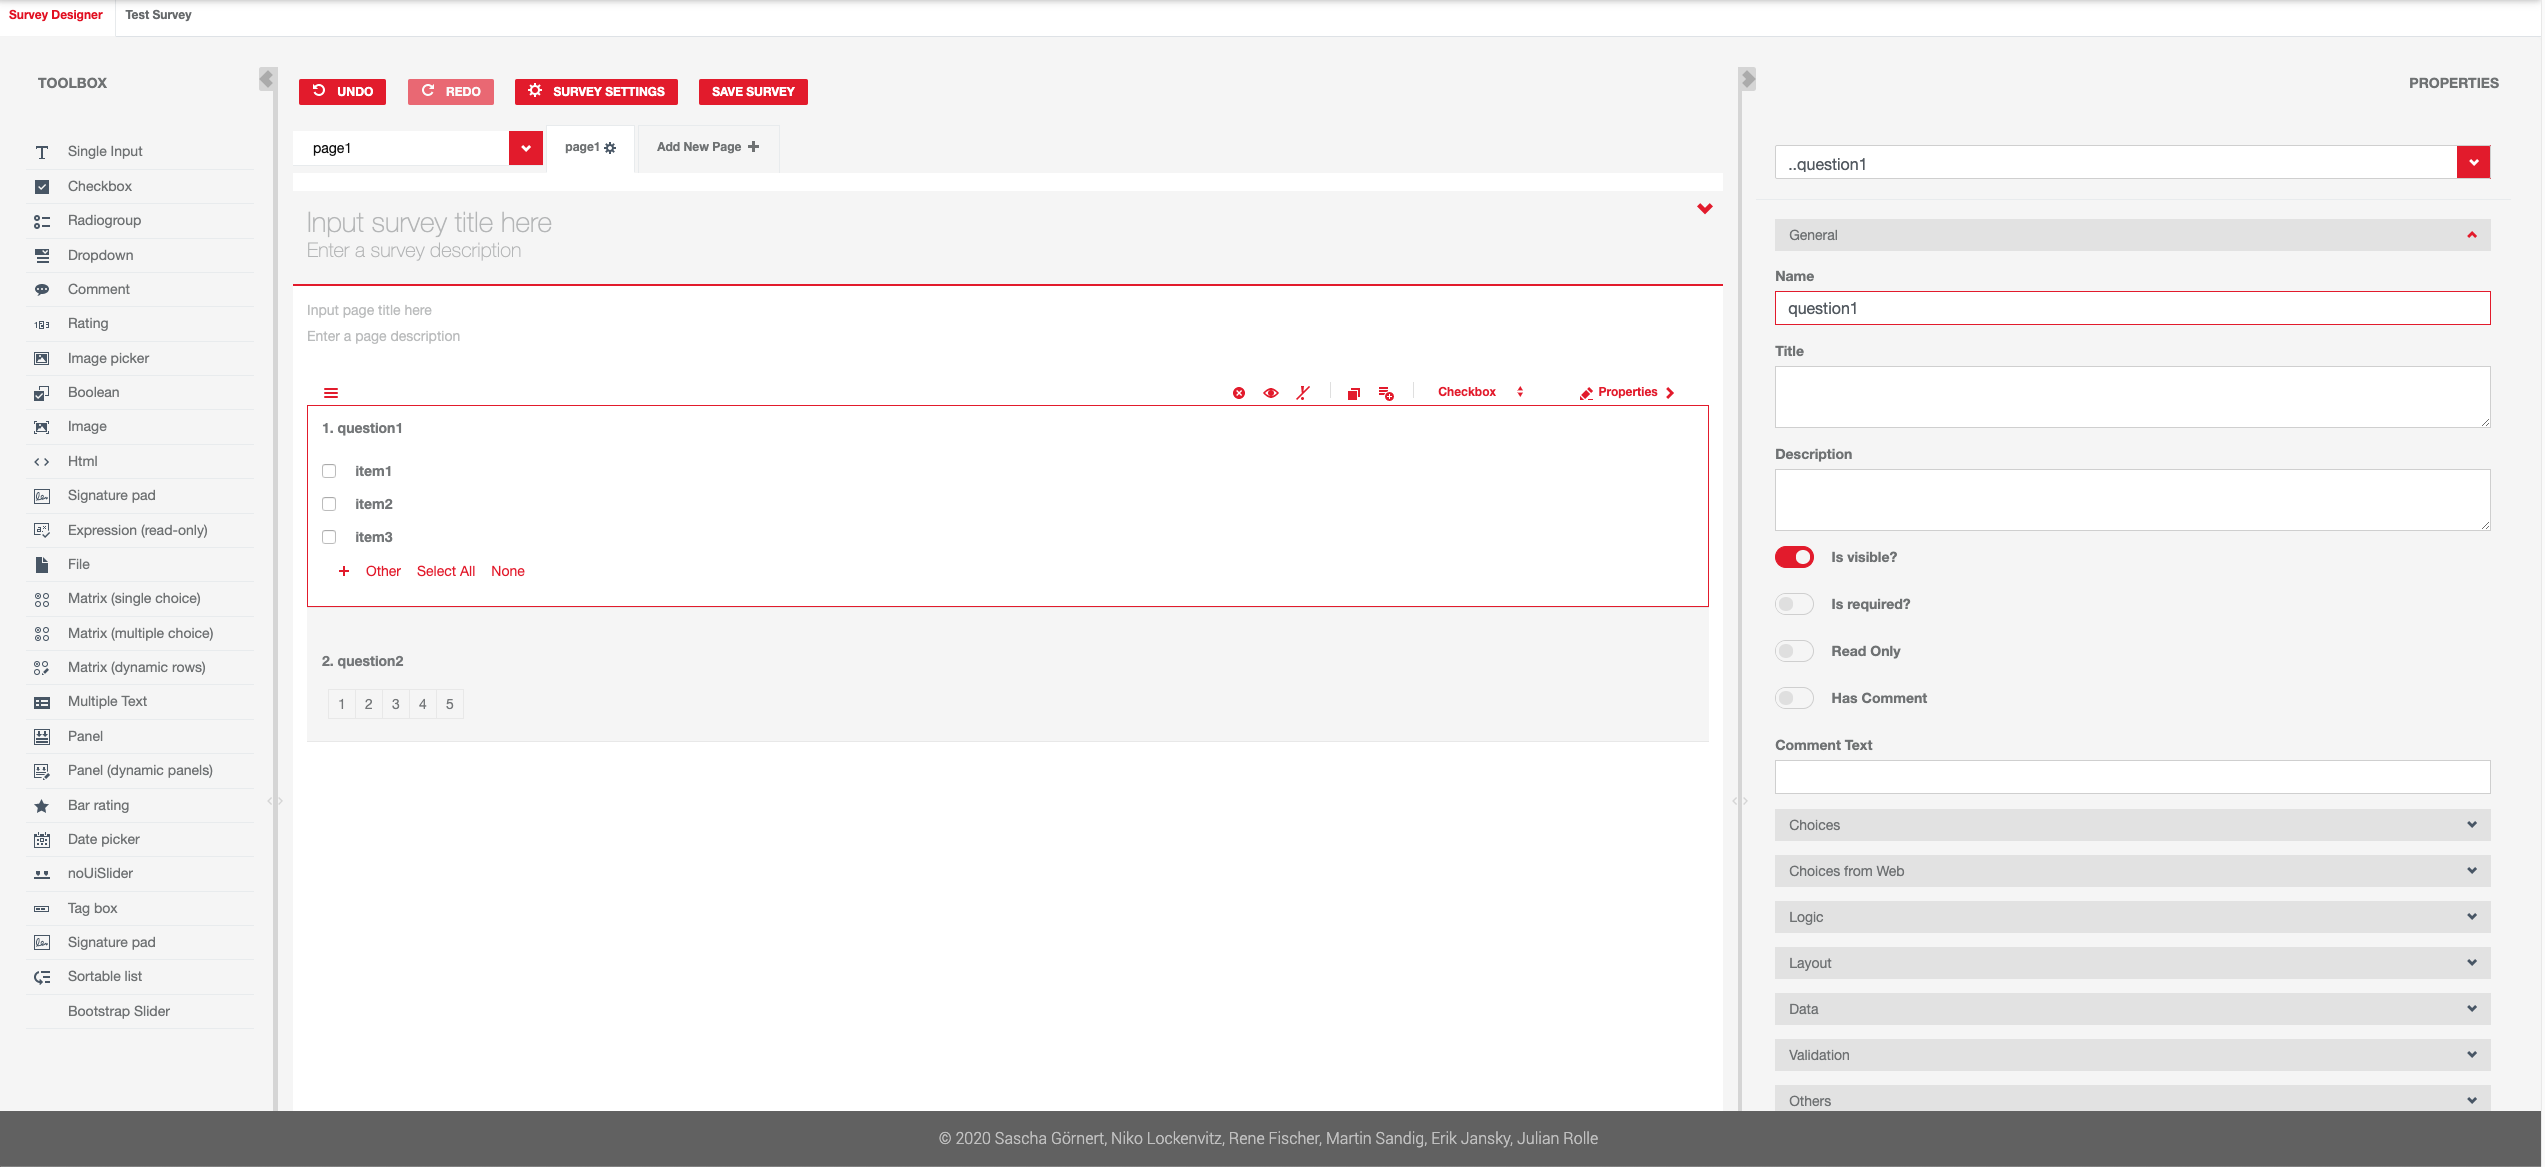
\includegraphics[width=0.95\textwidth, keepaspectratio]{img/client/CreateSurveyMaster.png}
	\captionsetup{justification=centering, format=plain}
	\caption[\acf{UI}: Erstellen einer Umfrage]{\acf{UI}: Erstellen einer Umfrage \\ \quelleScreenshot}
	\label{fig:SurveyCreatorImplement}
\end{figure}

Klickt der Benutzer auf die Schaltfläche \jinline|Test Survey|, kann er seine erstellte Survey ansehen, wie sie sich auf verschiedene Geräte wie \zb iPhone 8 verhält.
\abb \vref{fig:SurveyAnsicht} zeigt die Möglichkeit, sich seine erstellte Survey auf einem bestimmten Gerät \engl{device} anzuschauen (hier: Desktop).  
Der Benutzer hat die Möglichkeit über eine \emph{preview} wie in \abb \vref{fig:SurveyMobileAnsicht} verschiedene mobile Geräte auszuwählen, um auch auf diesen Geräten die Darstellung seiner Umfrage zu überprüfen. 
\abb \vref{fig:SurveyMobileAnsichtIPhone8} zeigt die erstellte Umfrage auf einem iPhone 8 an wohingegen \abb \vref{fig:SurveyMobileAnsichtAndroid}. 


\begin{figure}[h]
	\centering
	\captionsetup{justification=centering, format=plain}
	\subfigure[Ansicht der Survey]{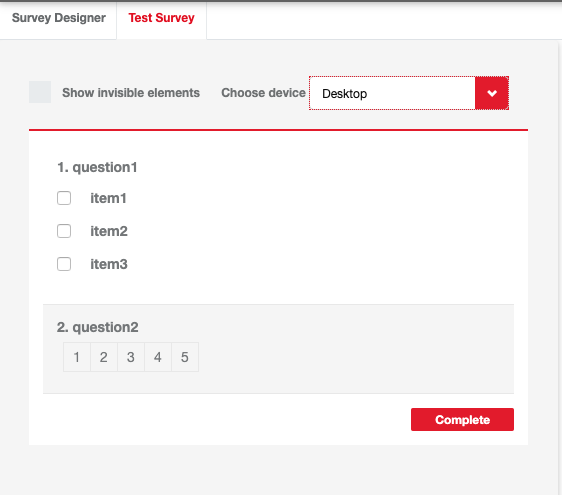
\includegraphics[width=0.48\textwidth]{img/client/CreateSurveyMaster_View1.png}\label{fig:SurveyAnsicht}}\hfill
	\subfigure[Auswahl der verschiedenen Mobileansichten]{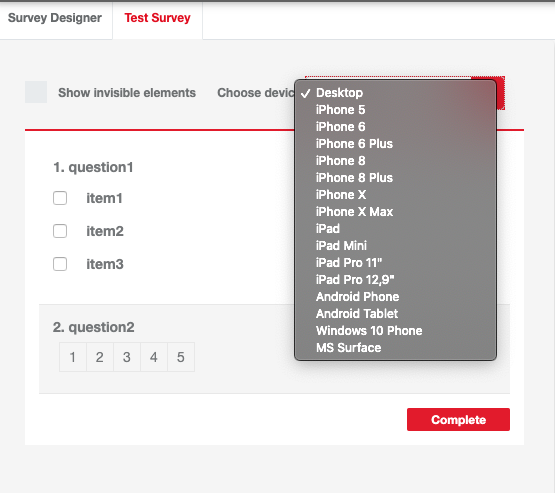
\includegraphics[width=0.48\textwidth]{img/client/CreateSurveyMaster_View2.png}\label{fig:SurveyMobileAnsicht}}\hfill
	\subfigure[Mobileansicht: iPhone 8]{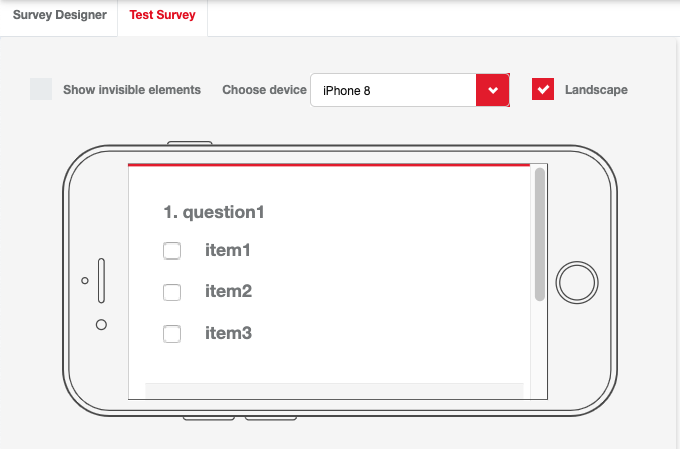
\includegraphics[width=0.48\textwidth]{img/client/CreateSurveyMaster_View3.png}\label{fig:SurveyMobileAnsichtIPhone8}}\hfill
	\subfigure[Mobileansicht: Android Phone]{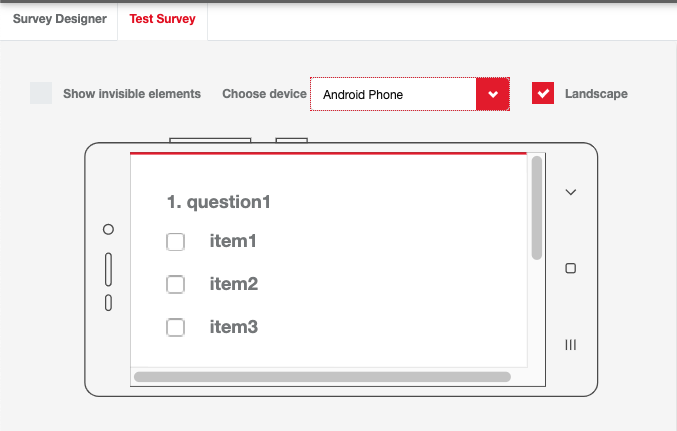
\includegraphics[width=0.48\textwidth]{img/client/CreateSurveyMaster_View4.png}\label{fig:SurveyMobileAnsichtAndroid}}
	\caption[Ansichtsoberfläche der Umfrage]{\label{fig:SurveyCreatorViewImplement}Ansichtsoberfläche der Umfrage \\ \quelleScreenshot}
\end{figure}

Über einen Button \jinline|Save Survey| kann der Benutzer die Umfrage speichern.
Er erhält auch hier wieder ein visuelles Feedback über den Erfolg oder Nichterfolg des Erstellens der Umfrage. 
Seine erstellte Umfragen erscheint in seinen \emph{Survey Dashboard} (Kap. \vref{ssec:UmfrageDashboard}).
